\RequirePackage[2020-02-02]{latexrelease}
\documentclass[conference]{IEEEtran}
\IEEEoverridecommandlockouts
% The preceding line is only needed to identify funding in the first footnote. If that is unneeded, please comment it out.

\usepackage{xcolor}
\usepackage[hang, flushmargin]{footmisc}
\usepackage[
colorlinks=false, % don't highlight links in color
linkbordercolor=green, % set border color for internal links
citebordercolor=green, % set border color for citations
filebordercolor=magenta, % set border color for file links
urlbordercolor=cyan, % set border color for URLs
pdfborder={0 0 1}, % determine border around links
linkcolor=black,
citecolor=black,
filecolor=black,
urlcolor=black,
]{hyperref}
\usepackage{footnotebackref}

\usepackage{cite}
\usepackage{amsmath,amssymb,amsfonts}
\usepackage{algorithmic}
\usepackage{graphicx}
\usepackage{textcomp}

\def\BibTeX{{\rm B\kern-.05em{\sc i\kern-.025em b}\kern-.08em
    T\kern-.1667em\lower.7ex\hbox{E}\kern-.125emX}}

\usepackage[english]{babel}
\addto\extrasenglish{  
    \def\figureautorefname{Figure}
    \def\tableautorefname{Table}
    \def\algorithmautorefname{Algorithm}
    \def\sectionautorefname{Section}
    \def\subsectionautorefname{Subsection}
}

\newcommand{\supertiny}{\fontsize{1}{2}\selectfont}

\usepackage{catoptions}
\makeatletter

\def\Autoref#1{%
  \begingroup
  \edef\reserved@a{\cpttrimspaces{#1}}%
  \ifcsndefTF{r@#1}{%
    \xaftercsname{\expandafter\testreftype\@fourthoffive}
      {r@\reserved@a}.\\{#1}%
  }{%
    \ref{#1}%
  }%
  \endgroup
}
\def\testreftype#1.#2\\#3{%
  \ifcsndefTF{#1autorefname}{%
    \def\reserved@a##1##2\@nil{%
      \uppercase{\def\ref@name{##1}}%
      \csn@edef{#1autorefname}{\ref@name##2}%
      \autoref{#3}%
    }%
    \reserved@a#1\@nil
  }{%
    \autoref{#3}%
  }%
}
\makeatother

\usepackage[T1]{fontenc}
\usepackage{graphicx}
%\usepackage{color}
%\renewcommand\UrlFont{\color{blue}\rmfamily}

\usepackage{amsmath,amssymb,amsfonts}
\usepackage[inline, shortlabels]{enumitem}
\usepackage{tabularx}
\usepackage{caption}
\usepackage{listings}
% \usepackage{titlesec}
\usepackage{ragged2e}

\usepackage{xurl}
% \usepackage[hyphens]{url}
\usepackage{pifont}
\usepackage{multirow}
\usepackage[linesnumbered,ruled,vlined]{algorithm2e}
\usepackage{float}
\usepackage{listings}
\usepackage{xcolor}

\definecolor{codegreen}{rgb}{0,0.6,0}
\definecolor{codegray}{rgb}{0.5,0.5,0.5}
\definecolor{codepurple}{rgb}{0.58,0,0.82}
\definecolor{backcolour}{rgb}{0.95,0.95,0.92}
 
\lstdefinestyle{mystyle}{
    backgroundcolor=\color{backcolour},   
    commentstyle=\color{codegreen},
    keywordstyle=\color{magenta},
    numberstyle=\tiny\color{codegray},
    stringstyle=\color{codepurple},
    basicstyle=\footnotesize,
    breakatwhitespace=false,         
    breaklines=true,                 
    captionpos=b,                    
    keepspaces=true,                 
    numbers=left,                    
    numbersep=5pt,                  
    showspaces=false,                
    showstringspaces=false,
    showtabs=false,                  
    tabsize=2
}
 
\lstset{style=mystyle}

% --- Tickz
\usepackage{physics}
\usepackage{amsmath}
\usepackage{tikz}
\usepackage{mathdots}
\usepackage{yhmath}
\usepackage{cancel}
\usepackage{color}
\usepackage{siunitx}
\usepackage{array}
\usepackage{multirow}
\usepackage{amssymb}
\usepackage{gensymb}
\usepackage{tabularx}
\usepackage{extarrows}
\usepackage{booktabs}
\usetikzlibrary{fadings}
\usetikzlibrary{patterns}
\usetikzlibrary{shadows.blur}
\usetikzlibrary{shapes}

% ---------
% \usepackage{titlesec}
\usepackage{pdfpages}
\usepackage{booktabs}
\usepackage{csquotes}
\usepackage{lipsum}  
\usepackage{arydshln}
\usepackage{smartdiagram}
\usepackage{textcomp}
\usepackage{tabularray}\UseTblrLibrary{varwidth}
\usepackage{xcolor}
\def\BibTeX{{\rm B\kern-.05em{\sc i\kern-.025em b}\kern-.08em
    T\kern-.1667em\lower.7ex\hbox{E}\kern-.125emX}}
\usepackage{cite}
\usepackage{amsmath}
\newcommand{\probP}{\text{I\kern-0.15em P}}
\usepackage{etoolbox}
\patchcmd{\thebibliography}{\section*{\refname}}{}{}{}

\setlength\tabcolsep{0.5pt}

\newcommand{\before}[1]{\textcolor{red}{#1}}
\newcommand{\after}[1]{\textcolor{green}{#1}}

\newcommand{\old}[1]{\textcolor{orange}{#1}}
\newcommand{\rem}[1]{\textcolor{red}{#1}}
\newcommand{\todo}[1]{\textcolor{orange}{\newline \textit{\textbf{TODO:} #1}} \newline \newline }



\newcounter{relation}
\setcounter{relation}{0}
\renewcommand{\therelation}{\arabic{relation}}
\newcommand{\relationautorefname}{Relation}

\newenvironment{relation}[1][]{%
    \refstepcounter{relation}%
    \noindent \raggedright \textit{\textbf{Relation. \therelation}} \hfill$}
{%
$ \hfill \phantom{x}

}

\makeatletter
\newcommand{\linebreakand}{%
  \end{@IEEEauthorhalign}
  \hfill\mbox{}\par
  \mbox{}\hfill\begin{@IEEEauthorhalign}
}
\makeatother

% =======================================

\begin{document}

\title{An Organization-oriented MARL Approach for Cyberdefense in a Drone Swarm Scenario}

\author{

    \IEEEauthorblockN{Julien Soulé}
    \IEEEauthorblockA{\textit{Thales Land and Air Systems, BU IAS}}
    %Rennes, France \\
    \IEEEauthorblockA{\textit{Univ. Grenoble Alpes,} \\
        \textit{Grenoble INP, LCIS, 26000,}\\
        Valence, France \\
        julien.soule@lcis.grenoble-inp.fr}

    \and

    \IEEEauthorblockN{Louis-Marie Traonouez}
    \IEEEauthorblockA{\textit{Thales LAS / IAS / La Ruche} \\
        Rennes, France \\
        louis-marie.traonouez@thalesgroup.com}

    % }

    % \and

    \linebreakand

    \hspace{1.8cm}
    \IEEEauthorblockN{Paul Théron}
    \IEEEauthorblockA{
        \hspace{1.8cm}
        \textit{AICA IWG} \\
        \hspace{1.8cm}
        La Guillermie, France \\
        %lieu-dit Le Bourg, France \\
        \hspace{1.8cm}
        paul.theron@orange.fr}

    \and

    \hspace{0.3cm}
    \IEEEauthorblockN{Jean-Paul Jamont\IEEEauthorrefmark{1}, Michel Occello\IEEEauthorrefmark{2}}
    \IEEEauthorblockA{
        \hspace{0.3cm}
        \textit{Univ. Grenoble Alpes,} \\
        \hspace{0.3cm}
        \textit{Grenoble INP, LCIS, 26000,}\\
        \hspace{0.3cm}
        Valence, France \\
        \hspace{0.3cm}
        \{\IEEEauthorrefmark{1}jean-paul.jamont,\IEEEauthorrefmark{2}michel.occello\}@lcis.grenoble-inp.fr
    }
}

% \IEEEauthorblockN{Michel Occello}
% \IEEEauthorblockA{\textit{Univ. Grenoble Alpes,} \\
% \textit{Grenoble INP, LCIS, 26000,}\\
% Valence, France \\
% michel.occello@lcis.grenoble-inp.fr}


\maketitle

\begin{abstract}
    Autonomous Cyberdefense is becoming increasingly essential for securing decentralized environments where centralized methods are impractical. Multi-Agent Reinforcement Learning (MARL) has shown potential in training agents to autonomously achieve Cyberdefense goals. However, it is not possible to fully predict or monitor agents' behavior. This limitation hinders the development of safe and fully autonomous Cyberdefense agents suitable for deployment in critical networked environments.
    %
    We propose a Cyberdefense-oriented algorithmic approach that constrains Cyberdefender agents' policies to specific roles and missions within a general Cyberdefense architecture. The core algorithm adapts the MARL framework to incorporate the $\mathcal{M}OISE^+$ organizational model.
    %    
    We apply our algorithm to a simulated Cyberdefense scenario involving a drone swarm facing malware attacks. The results show our approach does guide the training of agents to detect, mitigate, and eliminate malware. It results in more performant, safe, and stable collective strategies compared to regular MARL training.
    % This also contributes to enhance the swarm's resilience and operational effectiveness.
\end{abstract}

\begin{IEEEkeywords}
    Multi-Agent Reinforcement Learning, Cyberdefense, Drones, Autonomous Cyber Operation
\end{IEEEkeywords}

% ====================================================================================================

\section{Introduction}
\label{sec:introduction}

\textit{Autonomous Intelligent Cyberdefense Agents}~\cite{Kott2023} (AICA) are agents to be deployed in networked environments to detect, identify, and characterize anomalies/attacks, develop countermeasures, and execute them
%
\footnote{
    Theorized by the \textit{AICA International Work Group} (cf. \url{https://www.aica-iwg.org/}) and based on the results of NATO's \textit{Research Task Group IST-152}.
}.
Related AICA research highlights the increasing need for \textit{Autonomous Cyberdefense} to protect decentralized environments where traditional centralized approaches are ineffective, such as in IoT-based systems. A Multi-Agent System (MAS) offers robust and adaptive defense mechanisms by decomposing the complexity of Cyberdefense into sub-tasks delegated to collaborative agents deployed throughout the system.

The top-down approach involves designing Cyberdefense MAS from predefined architectures and functionalities. The \textit{MAS Centric AICA Reference Architecture} (MASCARA)~\cite{Kott2023} describes an AICA-like MAS with components that enable collaborative mechanisms based on explicitly defined plans or processes. However, this approach can be costly as it requires comprehensive knowledge of the deployment environment, which must be regularly updated due to frequent changes, such as topology modifications or new vulnerabilities.

The bottom-up approach may include Multi-Agent Reinforcement Learning (MARL)~\cite{Albrecht2024}, where agents learn to achieve Cyberdefense goals autonomously, enhancing MAS autonomy~\cite{hammar_stadle4_noms_23}. Despite promising simulation results, this approach lacks the safety guarantees necessary for real-world applications and does not provide explicit means to justify the MAS's success or failure~\cite{dulacarnold2019}. These issues hinder the development of fully or semi-autonomous Cyberdefense MAS, such as AICA, in critical environments, where actions must be justified given their potentially irreversible consequences.

To address this concern, we propose combining these two points of view by extending the \textit{Partial Relation between Agents' History and Organizational Model}~\cite{soule2024} (PRAHOM). PRAHOM is a general approach that enables integrating the $\mathcal{M}OISE^+$ organizational model into the MARL framework, laying the foundation for constraining learning. However, this perspective remains limited and faces scalability issues with the number of organizational specifications, which limits its application in complex networked environments.

The main contribution of this paper is the \textit{Cyberdefense-oriented PRAHOM} (CoPRAHOM) inspired by PRAHOM and related works. This algorithm is specifically intended to address Cyberdefense scenarios relying on general Cyberdefense architectures such as MASCARA. This algorithm enables users to constrain agents to Cyberdefense roles and missions. We implemented practical means to apply CoPRAHOM also aiming to address scalability concerns. One of the main interests is to ensure safety guarantees by embedding domain-specific knowledge, such as rules, or accelerating or stabilizing the training by restricting the search space.

We assessed CoPRAHOM in the simulated scenario provided by the 3rd CAGE Challenge~\cite{cage_challenge_3_announcement}. It involves creating a Cyberdefense MAS for detecting, mitigating, and eliminating malware programs in a drone swarm. Using CoPRAHOM, we developed several Cyberdefense MAS models. These models are used by CoPRAHOM to guide and constrain agents' training to better achieve the scenario's goals and ensure safety requirements. We verify that the trained agents exhibit expected collective strategies while being also fine-tuned throughout the training, making the overall score comparable to leading entries on the leaderboard.

The remainder of this paper is organized as follows. \Autoref{sec:marl_background} introduces the fundamentals of MARL. \Autoref{sec:related_works} reviews related works on MARL for Cyberdefense and agent training monitoring. \Autoref{sec:marl_moise_linking} outlines the $\mathcal{M}OISE^+$ model and its integration with MARL. \Autoref{sec:coprahom} describes the MASCARA architecture and the development of the CoPRAHOM algorithm. \Autoref{sec:coprahom_wrapper} details our \textit{Proof of Concept} (PoC) implementation of CoPRAHOM and its practical functionalities. \Autoref{sec:experimental_setup} covers the experimental setup for the 3rd CAGE Challenge and the evaluation metrics for CoPRAHOM. \Autoref{sec:results_and_discussion} presents and discusses the results. Finally, \Autoref{sec:conclusion} concludes the paper and outlines future research directions.


\section{MARL Background}\label{sec:marl_background}

Multi-Agent Reinforcement Learning (MARL) extends the principles of Reinforcement Learning (RL) to scenarios involving multiple interacting agents. Agents aim to maximize the overall cumulative reward through learning, but the presence of other agents introduces additional complexity due to the dynamic nature of the environment.

MARL is often modeled using the Decentralized Partially Observable Markov Decision Process (Dec-POMDP), a framework suitable for environments where agents have limited and differing observations. A Dec-POMDP is formally defined as a tuple $(S, \{A_i\}, T, R, \{\Omega_i\}, O, \gamma)$:

\begin{itemize}
    \item $S$: A finite set of states describing the environment.
    \item $\{A_i\}$: A set of action sets, one for each agent $i$.
    \item $T$: The state transition probability function $T(s, \vec{a}, s') = P(s'|s, \vec{a})$, where $\vec{a}$ is the joint action of all agents.
    \item $R$: The reward function $R(s, \vec{a}, s')$, mapping states and actions to a reward.
    \item $\{\Omega_i\}$: A set of observation sets, one for each agent $i$.
    \item $O$: The observation probability function $O(\vec{o} | s', \vec{a})$, where $\vec{o}$ is the joint observation of all agents.
    \item $\gamma \in [0,1]$: The discount factor for future rewards.
\end{itemize}

In MARL, each agent $i$ maintains a policy $\pi_i: H \times \Omega \rightarrow A$, mapping an action $a \in A$ from an observation $\omega \in \Omega$ and optionally the agent's history $h \in H, h=\langle(\omega_0,a_0),(\omega_1,a_1)\dots(\omega_{n_e},a_{n_e})\rangle$ (with $n_e \in \mathbb{N}$, the number of steps per episode). A joint policy $\pi_{\text{joint}} = (\pi_1, \pi_2, \ldots, \pi_n)$ describes the behavior of all agents collectively.

The ultimate goal is to find a joint policy $\pi_{\text{joint}}$ that maximizes the expected cumulative reward $U(\pi^*_{\text{joint}}) = \mathbb{E}\left[\sum_{t=0}^{\infty} \gamma^t R(s_t, \vec{a}_t)\right]$. Instead of solely aiming for a global optimum, our approach emphasizes obtaining approximate solutions with sufficient reward.

Various approaches enable solving Multi-Agent Reinforcement Learning (MARL) problems. \textbf{Value-based} methods, such as QMIX~\cite{rashid2018}, estimate the value function $Q(s,\vec{a})$ that indicates the expected cumulative reward for a given state $s$ and joint action $\vec{a}$. \textbf{Policy-based} methods, including Multi-Agent Proximal Policy Optimization~\cite{yu2022surprising} (MAPPO) and Multi-Agent Deep Deterministic Policy Gradient~\cite{lowe2017multi} (MADDPG), directly parameterize the policy as $\pi_\theta$ to optimize it possibly using centralized training and decentralized execution. \textbf{Actor-Critic} methods combine value-based and policy-based approaches, such as in COMA (Counterfactual Multi-Agent Policy Gradients) where the actor updates the policy parameters in the direction indicated by the critic, which evaluates the current policy.

\section{Related Works}
\label{sec:related_works}

We define organizational-oriented MARL as the broad field of research encompassing studies that introduce explicit specifications (such as rules, roles, or protocols) to guide or restrict the MARL training process to meet requirements. While the explicit integration of organizational specifications in MARL is not extensively covered in the literature, several approaches have been proposed to embed some constraints within MAS to ensure that agents conform to specific requirements.

\textbf{Learning with Organizational Constraints} \quad
In \cite{cruz2020norms}, the authors present a method for incorporating norms into the learning algorithms of agents, ensuring that their behavior remains within acceptable bounds. Additionally, \cite{villatoro2011social} proposes a mechanism for agents to learn and adapt to social norms in dynamic environments, highlighting the importance of norm adaptation in MAS.

A relevant subset of work belongs to \emph{Specification-Guided Reinforcement Learning}, which aims to generate policies that accomplish specific tasks using external specifications to guide learning in achieving objectives under given constraints~\cite{Bansal2022}. Jothimurugan et al.~\cite{Jothimurugan2021} propose logical specification learning, exploiting the compositional structure of specifications to generate policies for complex tasks.

\textbf{Policy-Based Approaches} \quad
Policy-based approaches provide a way to enforce organizational constraints by defining explicit policies that govern agent behavior. In \cite{krupanski2015norm}, the use of normative policies is investigated to guide agent interactions and decision-making processes. Moreover, \cite{vos2020governing} explores the use of governance mechanisms to enforce compliance with organizational policies in decentralized systems.

\textbf{Frameworks Integrating Organizational Aspects} \quad
Wang et al.~\cite{Wang2020} introduce an approach in which similar emerging roles are encouraged to jointly specialize in specific tasks. Tosic et al.~\cite{Tosic2010} propose a framework for coordination based on the communication capabilities of multi-agent systems. Zheng et al.~\cite{Zheng2018} present a platform for MARL that aims to facilitate research on artificial collective intelligence by providing a comprehensive set of evaluation metrics to compare the performance of MARL algorithms.

% \textbf{Evaluation and Applications} \quad
% Several studies have evaluated the effectiveness of organizational models and policies in various applications. For example, \cite{dignum2004agent} evaluates the application of organizational models in e-commerce systems, demonstrating their utility in ensuring reliable and predictable agent behavior. Similarly, \cite{andrighetto2013normative} investigates the role of normative systems in regulating agent behavior in collaborative environments.

\textbf{MARL in Cybersecurity and Autonomous Cyber Operations} \quad
MARL has also been applied in cybersecurity to develop autonomous systems capable of defending against cyber threats. Albrecht et al.~\cite{Albrecht2024} explore the use of MARL for training agents in dynamic environments to achieve cybersecurity goals.
% Kott et al.~\cite{Kott2023} discuss the deployment of AICA in networked environments to detect and mitigate cyber-attacks.
Similarly, in \cite{Hammar2022}, the authors present a framework for integrating digital twins with MARL to enhance cybersecurity automation.

Despite these advancements, there is still a scarcity of research explicitly utilizing organizational specifications to constrain agent learning in accordance with requirements. To our knowledge, no existing work facilitates the generation of a MAS that explicitly satisfies additional organizational constraints. CoPRAHOM's originality lies in using an organizational model explicitly as a general method for constraining learning based on these requirements.

\section{Combining $\mathcal{M}OISE^+$ Model with MARL}
\label{sec:marl_moise_linking}

This section presents principles for adapting MARL with organizational specifications, aligning policies with expected role behaviors and mission goals.

The $\mathcal{M}OISE^+$ model provides a structured framework for defining roles and interactions within a Multi-Agent System (MAS). It is compatible with MARL, allowing for formal descriptions of agent policies. The CoPRAHOM approach embeds $\mathcal{M}OISE^+$ specifications into MARL training, enabling agents to adhere to predefined roles and missions. $\mathcal{M}OISE^+$ defines \textbf{Organizational Specifications (OS)} as $\mathcal{OS} = \langle \mathcal{SS}, \mathcal{FS}, \mathcal{DS} \rangle$, where $\mathcal{SS}$ are \textbf{Structural Specifications}, $\mathcal{FS}$ are \textbf{Functional Specifications}, and $\mathcal{DS}$ are \textbf{Deontic Specifications}.

\subsection{Structural Specifications and Policy Constraints}

\textbf{Structural Specifications} ($\mathcal{SS} = \langle \mathcal{R}, \mathcal{IR}, \mathcal{G} \rangle$) describe organizational structure:
\begin{itemize}
    \item $\mathcal{R}_{ss}$: All roles ($\rho \in \mathcal{R}$).
    \item $\mathcal{IR}$: Role inheritance relation ($\rho_1 \sqsubset \rho_2$).
    \item $\mathcal{RG} \subseteq \mathcal{GR}$: Root groups, $\mathcal{GR} = \langle \mathcal{R}, \mathcal{SG}, \mathcal{L}^{intra}, \mathcal{L}^{inter}, \mathcal{C}^{intra}, \mathcal{C}^{inter}, np, ng \rangle$, where:
    \begin{itemize}
        \item $\mathcal{R}$: Non-abstract roles.
        \item $\mathcal{SG}$: Sub-groups.
        \item $\mathcal{L}$: Links $(\rho_s, \rho_d, t)$, where $t \in \{acq, com, aut\}$.
        \item $\mathcal{L}^{intra}$: Intra-group links.
        \item $\mathcal{L}^{inter}$: Inter-group links.
        \item $\mathcal{C}$: Compatibilities $(\rho_a \bowtie \rho_b)$.
        \item $\mathcal{C}^{intra}$: Intra-group compatibilities.
        \item $\mathcal{C}^{inter}$: Inter-group compatibilities.
        \item $np$: Cardinality of agents in a role.
        \item $ng$: Cardinality of each sub-group.
    \end{itemize}
\end{itemize}

Direct policy constraints are impractical due to black-box models like neural networks. Instead, we represent roles as history subsets $\mathcal{P}(H)$ that agents should generate, characterizing expected behaviors. Each role maps to a history subset via $rh: \mathcal{R} \rightarrow \mathcal{P}(H)$. Agents' policies should generate histories belonging to these subsets.

We address large, complex observations by using labels to represent observations. The mapping $ol: \mathcal{P}(\Omega) \rightarrow \mathcal{P}(L)$ translates observations to labels, potentially using a trained Large Language Model (LLM). This simplifies defining history subsets, which can be represented by patterns, rules, or custom scripts.

\begin{figure}[h!]
    \centering
    


\tikzset{every picture/.style={line width=0.75pt}} %set default line width to 0.75pt        

\begin{tikzpicture}[x=0.75pt,y=0.75pt,yscale=-1,xscale=1]
%uncomment if require: \path (0,1800); %set diagram left start at 0, and has height of 1800

%Shape: Rectangle [id:dp9341453924522656] 
\draw  [fill={rgb, 255:red, 255; green, 255; blue, 255 }  ,fill opacity=1 ] (160,44) -- (510,44) -- (510,167) -- (160,167) -- cycle ;
%Shape: Rectangle [id:dp4628140741854456] 
\draw  [fill={rgb, 255:red, 184; green, 233; blue, 134 }  ,fill opacity=0.34 ] (374,52) -- (504,52) -- (504,162) -- (374,162) -- cycle ;
%Shape: Rectangle [id:dp6461749357206974] 
\draw  [fill={rgb, 255:red, 184; green, 233; blue, 134 }  ,fill opacity=0.34 ] (378,78) -- (500,78) -- (500,158) -- (378,158) -- cycle ;
%Shape: Rectangle [id:dp47018118728898073] 
\draw  [fill={rgb, 255:red, 248; green, 231; blue, 28 }  ,fill opacity=0.4 ] (164,48) -- (314,48) -- (314,162) -- (164,162) -- cycle ;
%Straight Lines [id:da37904402438854] 
\draw    (400,150.31) -- (400,193.69) ;
\draw [shift={(400,195.69)}, rotate = 270] [color={rgb, 255:red, 0; green, 0; blue, 0 }  ][line width=0.75]    (10.93,-3.29) .. controls (6.95,-1.4) and (3.31,-0.3) .. (0,0) .. controls (3.31,0.3) and (6.95,1.4) .. (10.93,3.29)   ;
\draw [shift={(400,148.31)}, rotate = 90] [color={rgb, 255:red, 0; green, 0; blue, 0 }  ][line width=0.75]    (10.93,-3.29) .. controls (6.95,-1.4) and (3.31,-0.3) .. (0,0) .. controls (3.31,0.3) and (6.95,1.4) .. (10.93,3.29)   ;
%Straight Lines [id:da30557994145553513] 
\draw    (368,140) -- (386,140) ;
\draw [shift={(388,140)}, rotate = 180] [color={rgb, 255:red, 0; green, 0; blue, 0 }  ][line width=0.75]    (10.93,-3.29) .. controls (6.95,-1.4) and (3.31,-0.3) .. (0,0) .. controls (3.31,0.3) and (6.95,1.4) .. (10.93,3.29)   ;
%Shape: Rectangle [id:dp15689957472567295] 
\draw  [fill={rgb, 255:red, 248; green, 231; blue, 28 }  ,fill opacity=0.4 ] (169.56,76) -- (309.06,76) -- (309.06,157) -- (169.56,157) -- cycle ;
%Shape: Rectangle [id:dp6202366628126772] 
\draw  [fill={rgb, 255:red, 255; green, 255; blue, 255 }  ,fill opacity=1 ] (372,196) -- (414,196) -- (414,216) -- (372,216) -- cycle ;

%Shape: Rectangle [id:dp20067598884831228] 
\draw  [fill={rgb, 255:red, 248; green, 231; blue, 28 }  ,fill opacity=0.4 ] (212.06,129) -- (234.06,129) -- (234.06,149) -- (212.06,149) -- cycle ;

%Shape: Rectangle [id:dp5970765798398485] 
\draw  [fill={rgb, 255:red, 248; green, 231; blue, 28 }  ,fill opacity=0.4 ] (178.06,129) -- (203.06,129) -- (203.06,149) -- (178.06,149) -- cycle ;
%Shape: Rectangle [id:dp92237875722883] 
\draw  [fill={rgb, 255:red, 248; green, 231; blue, 28 }  ,fill opacity=0.4 ] (178.06,102) -- (218.06,102) -- (218.06,122) -- (178.06,122) -- cycle ;

%Shape: Rectangle [id:dp6591761395302378] 
\draw  [fill={rgb, 255:red, 248; green, 231; blue, 28 }  ,fill opacity=0.4 ] (178.06,80) -- (218.06,80) -- (218.06,100) -- (178.06,100) -- cycle ;

%Shape: Rectangle [id:dp11794703752595392] 
\draw  [fill={rgb, 255:red, 248; green, 231; blue, 28 }  ,fill opacity=0.4 ] (258.5,80) -- (298.5,80) -- (298.5,100) -- (258.5,100) -- cycle ;

%Shape: Rectangle [id:dp6557958558103134] 
\draw  [fill={rgb, 255:red, 248; green, 231; blue, 28 }  ,fill opacity=0.4 ] (259,102) -- (299,102) -- (299,122) -- (259,122) -- cycle ;

%Shape: Rectangle [id:dp8284992701408749] 
\draw  [fill={rgb, 255:red, 65; green, 117; blue, 5 }  ,fill opacity=1 ] (388,129) -- (410,129) -- (410,149) -- (388,149) -- cycle ;

%Shape: Rectangle [id:dp7066110016250453] 
\draw  [fill={rgb, 255:red, 248; green, 231; blue, 28 }  ,fill opacity=0.4 ] (244,129) -- (266,129) -- (266,149) -- (244,149) -- cycle ;

%Shape: Rectangle [id:dp4021333114319714] 
\draw  [fill={rgb, 255:red, 248; green, 231; blue, 28 }  ,fill opacity=0.4 ] (170.31,53) -- (195.69,53) -- (195.69,73) -- (170.31,73) -- cycle ;

%Shape: Rectangle [id:dp8476756388266236] 
\draw  [fill={rgb, 255:red, 248; green, 231; blue, 28 }  ,fill opacity=0.4 ] (200,53) -- (226,53) -- (226,73) -- (200,73) -- cycle ;

%Shape: Rectangle [id:dp07470576340681823] 
\draw  [fill={rgb, 255:red, 74; green, 144; blue, 226 }  ,fill opacity=1 ] (324,101) -- (364,101) -- (364,121) -- (324,121) -- cycle ;

%Shape: Rectangle [id:dp31407652093057714] 
\draw  [fill={rgb, 255:red, 74; green, 144; blue, 226 }  ,fill opacity=1 ] (324,129) -- (364,129) -- (364,149) -- (324,149) -- cycle ;

%Shape: Rectangle [id:dp053729126169398844] 
\draw  [fill={rgb, 255:red, 184; green, 233; blue, 134 }  ,fill opacity=0.34 ] (378,55) -- (404,55) -- (404,75) -- (378,75) -- cycle ;

%Shape: Rectangle [id:dp7720103442630182] 
\draw  [fill={rgb, 255:red, 184; green, 233; blue, 134 }  ,fill opacity=0.34 ] (405.94,103) -- (431.94,103) -- (431.94,123) -- (405.94,123) -- cycle ;

%Shape: Rectangle [id:dp3183552657000306] 
\draw  [fill={rgb, 255:red, 184; green, 233; blue, 134 }  ,fill opacity=0.34 ] (447.44,103) -- (473.44,103) -- (473.44,123) -- (447.44,123) -- cycle ;

%Shape: Rectangle [id:dp10802424702469593] 
\draw  [fill={rgb, 255:red, 184; green, 233; blue, 134 }  ,fill opacity=0.34 ] (466,129) -- (488,129) -- (488,149) -- (466,149) -- cycle ;

%Shape: Rectangle [id:dp16589412198505937] 
\draw  [fill={rgb, 255:red, 184; green, 233; blue, 134 }  ,fill opacity=0.34 ] (428,129) -- (450,129) -- (450,149) -- (428,149) -- cycle ;

%Shape: Rectangle [id:dp1270989692188249] 
\draw  [fill={rgb, 255:red, 255; green, 255; blue, 255 }  ,fill opacity=1 ] (258,196) -- (300,196) -- (300,216) -- (258,216) -- cycle ;

%Straight Lines [id:da40017392935840324] 
\draw    (286,149.69) -- (286,193.69) ;
\draw [shift={(286,195.69)}, rotate = 270] [color={rgb, 255:red, 0; green, 0; blue, 0 }  ][line width=0.75]    (10.93,-3.29) .. controls (6.95,-1.4) and (3.31,-0.3) .. (0,0) .. controls (3.31,0.3) and (6.95,1.4) .. (10.93,3.29)   ;
\draw [shift={(286,147.69)}, rotate = 90] [color={rgb, 255:red, 0; green, 0; blue, 0 }  ][line width=0.75]    (10.93,-3.29) .. controls (6.95,-1.4) and (3.31,-0.3) .. (0,0) .. controls (3.31,0.3) and (6.95,1.4) .. (10.93,3.29)   ;
%Shape: Rectangle [id:dp21027747628033966] 
\draw  [fill={rgb, 255:red, 245; green, 166; blue, 35 }  ,fill opacity=1 ] (276,129) -- (298,129) -- (298,149) -- (276,149) -- cycle ;

%Shape: Rectangle [id:dp5582162899072272] 
\draw  [fill={rgb, 255:red, 255; green, 255; blue, 255 }  ,fill opacity=1 ] (172,178) -- (184,178) -- (184,190) -- (172,190) -- cycle ;
%Straight Lines [id:da3472969066473863] 
\draw    (170,210) -- (192,210) ;
\draw [shift={(194,210)}, rotate = 180] [color={rgb, 255:red, 0; green, 0; blue, 0 }  ][line width=0.75]    (6.56,-1.97) .. controls (4.17,-0.84) and (1.99,-0.18) .. (0,0) .. controls (1.99,0.18) and (4.17,0.84) .. (6.56,1.97)   ;
\draw [shift={(168,210)}, rotate = 0] [color={rgb, 255:red, 0; green, 0; blue, 0 }  ][line width=0.75]    (6.56,-1.97) .. controls (4.17,-0.84) and (1.99,-0.18) .. (0,0) .. controls (1.99,0.18) and (4.17,0.84) .. (6.56,1.97)   ;
%Shape: Rectangle [id:dp07012270906311535] 
\draw  [fill={rgb, 255:red, 255; green, 255; blue, 255 }  ,fill opacity=1 ] (332,197) -- (354,197) -- (354,217) -- (332,217) -- cycle ;

%Straight Lines [id:da7534392810513293] 
\draw    (344,164) -- (344,194) ;
\draw [shift={(344,196)}, rotate = 270] [color={rgb, 255:red, 0; green, 0; blue, 0 }  ][line width=0.75]    (10.93,-3.29) .. controls (6.95,-1.4) and (3.31,-0.3) .. (0,0) .. controls (3.31,0.3) and (6.95,1.4) .. (10.93,3.29)   ;
\draw [shift={(344,162)}, rotate = 90] [color={rgb, 255:red, 0; green, 0; blue, 0 }  ][line width=0.75]    (10.93,-3.29) .. controls (6.95,-1.4) and (3.31,-0.3) .. (0,0) .. controls (3.31,0.3) and (6.95,1.4) .. (10.93,3.29)   ;
%Straight Lines [id:da4125176624573814] 
\draw    (320,140) -- (300,140) ;
\draw [shift={(298,140)}, rotate = 360] [color={rgb, 255:red, 0; green, 0; blue, 0 }  ][line width=0.75]    (10.93,-3.29) .. controls (6.95,-1.4) and (3.31,-0.3) .. (0,0) .. controls (3.31,0.3) and (6.95,1.4) .. (10.93,3.29)   ;
%Shape: Rectangle [id:dp005426842763594397] 
\draw  [fill={rgb, 255:red, 80; green, 227; blue, 194 }  ,fill opacity=0.36 ] (320,76) -- (368,76) -- (368,162) -- (320,162) -- cycle ;
%Straight Lines [id:da9128713017721406] 
\draw    (478,150.31) -- (478,193.69) ;
\draw [shift={(478,195.69)}, rotate = 270] [color={rgb, 255:red, 0; green, 0; blue, 0 }  ][line width=0.75]    (10.93,-3.29) .. controls (6.95,-1.4) and (3.31,-0.3) .. (0,0) .. controls (3.31,0.3) and (6.95,1.4) .. (10.93,3.29)   ;
\draw [shift={(478,148.31)}, rotate = 90] [color={rgb, 255:red, 0; green, 0; blue, 0 }  ][line width=0.75]    (10.93,-3.29) .. controls (6.95,-1.4) and (3.31,-0.3) .. (0,0) .. controls (3.31,0.3) and (6.95,1.4) .. (10.93,3.29)   ;
%Shape: Rectangle [id:dp7604827971406838] 
\draw  [fill={rgb, 255:red, 255; green, 255; blue, 255 }  ,fill opacity=1 ] (450,196) -- (492,196) -- (492,216) -- (450,216) -- cycle ;



% Text Node
\draw (465,179) node   [align=left] {$gh$};
% Text Node
\draw (181.5,204) node  [font=\tiny] [align=left] {$name$};
% Text Node
\draw (334,179) node   [align=left] {$da$};
% Text Node
\draw (222,207) node  [font=\footnotesize] [align=left] {\begin{minipage}[lt]{29.67pt}\setlength\topsep{0pt}
\begin{center}
{\small Relation}
\end{center}

\end{minipage}};
% Text Node
\draw (202,185) node  [font=\footnotesize] [align=left] {\begin{minipage}[lt]{13.75pt}\setlength\topsep{0pt}
\begin{center}
{\small Set}
\end{center}

\end{minipage}};
% Text Node
\draw (343.5,61) node   [align=left] {$\mathcal{OS}$};
% Text Node
\draw (190.56,139) node   [align=left] {$\mathcal{SG}$};
% Text Node
\draw (345,85) node   [align=left] {$\mathcal{DS}$};
% Text Node
\draw (245.5,61) node   [align=left] {$\mathcal{SS}$};
% Text Node
\draw (387,179) node   [align=left] {$mh$};
% Text Node
\draw (275.5,177) node   [align=left] {$rh$};
% Text Node
\draw (237.56,91) node   [align=left] {$\mathcal{G}r$};
% Text Node
\draw (440.5,65) node   [align=left] {$\mathcal{FS}$};
% Text Node
\draw (439.44,90) node   [align=left] {$\mathcal{SCH}$};
% Text Node
\draw (472,205) node   [align=left] {$\mathcal{P}(H)$};
% Text Node
\draw (343,207) node   [align=left] {$\mathcal{A}$};
% Text Node
\draw (287,139) node   [align=left] {$\mathcal{R}$};
% Text Node
\draw (280,205) node   [align=left] {$\mathcal{P}(H)$};
% Text Node
\draw (439,139) node   [align=left] {$\mathcal{P}$};
% Text Node
\draw (477,139) node   [align=left] {$\mathcal{G}$};
% Text Node
\draw (460.44,113) node   [align=left] {$nm$};
% Text Node
\draw (418.94,113) node   [align=left] {$mo$};
% Text Node
\draw (391,65) node   [align=left] {$\mathcal{PO}$};
% Text Node
\draw (345,139) node   [align=left] {$\mathcal{OBL}$};
% Text Node
\draw (345,111) node   [align=left] {$\mathcal{PER}$};
% Text Node
\draw (214,62) node   [align=left] {$\mathcal{R}_{ss}$};
% Text Node
\draw (183,63) node   [align=left] {$\mathcal{IR}$};
% Text Node
\draw (255,139) node   [align=left] {$\mathnormal{ng}$};
% Text Node
\draw (399,139) node   [align=left] {$\mathcal{M}$};
% Text Node
\draw (280,112) node   [align=left] {$\mathcal{C}^{inter}$};
% Text Node
\draw (279.5,90) node   [align=left] {$\mathcal{C}^{intra}$};
% Text Node
\draw (199.06,90) node   [align=left] {$\mathcal{L}^{intra}$};
% Text Node
\draw (199.06,112) node   [align=left] {$\mathcal{L}^{inter}$};
% Text Node
\draw (223.06,139) node   [align=left] {$np$};
% Text Node
\draw (394,205) node   [align=left] {$\mathcal{P}(H)$};


\end{tikzpicture}
    \caption{Relations between organizational specifications and history subsets}
    \label{fig:PRAHOM_osm_rels}
\end{figure}

A history subset constrains a policy to a role. We introduce \textbf{observable policy constraints} $c\pi: H \times \Omega \rightarrow \mathcal{P}(A)$, dictating allowable actions per observation. These constraints integrate into policies in three modes:
\begin{itemize}
    \item \textbf{Correct}: Adjusts any chosen action $\pi(\omega)$ to an expected one in $c\pi(\omega)$, ensuring safety.
    \item \textbf{Penalize}: Adds a penalty for actions $\pi(\omega) \notin c\pi(\omega)$, encouraging agents to learn constraints.
    \item \textbf{Correct\_Policy}: Creates a \textbf{constrained policy} $\pi_c$ where $c\pi$ corrects $\pi$, ensuring internal safety.
\end{itemize}

\subsection{Functional Specifications and Policy Constraints}

\textbf{Functional Specifications} ($\mathcal{FS} = \langle \mathcal{SCH}, \mathcal{PO} \rangle$) define tasks and goals:
\begin{itemize}
    \item $\mathcal{SCH} = \langle \mathcal{G}, \mathcal{M}, \mathcal{P}, mo, nm \rangle$: Social schemes, where:
    \begin{itemize}
        \item $\mathcal{G}$: Global goals.
        \item $\mathcal{M}$: Mission labels.
        \item $\mathcal{P}$: Plans $(g_f, \{g_i\}_{0 \leq i \leq s}, op, ps)$.
        \item $mo$: Goals for each mission.
        \item $nm$: Cardinality of agents per mission.
    \end{itemize}
    \item $\mathcal{PO}$: Preference orders $(m_1 \prec m_2)$.
\end{itemize}

Goals are represented as history subsets, $gh: \mathcal{G} \rightarrow \mathcal{P}(H)$. Missions map to expected histories $mh: \mathcal{M} \rightarrow \mathcal{P}(H)$. Goals impact MARL by updating the reward function, enticing agents to generate desired histories. We introduce \textbf{observable reward functions} $R_g: H \rightarrow \mathbb{R}$, measuring the closeness of generated histories to expected ones. Mission rewards are weighted sums of goal rewards, promoting faster convergence.

\subsection{Deontic Specifications and Policy Constraints}

\textbf{Deontic Specifications} ($\mathcal{DS} = \langle \mathcal{OBL}, \mathcal{PER} \rangle$) define permissions and obligations:
\begin{itemize}
    \item $\mathcal{TC}$: Time constraints.
    \item $\mathcal{OBL}$: Obligations $(obl(\rho_a, m, tc))$.
    \item $\mathcal{PER}$: Permissions $(per(\rho_a, m, tc))$.
\end{itemize}

The relation $da: \mathcal{PER} \cup \mathcal{OBL} \rightarrow \mathcal{P}(\mathcal{A})$ constrains roles and missions with time limits, managed by $dttl: \mathcal{PER} \cup \mathcal{OBL} \times \mathcal{A} \rightarrow \mathbb{N}$. Obligations have higher reward multipliers than permissions, prioritizing mission adherence.

These principles integrate organizational specifications into the MARL framework, forming the PRAHOM algorithm.

\section{A Cyberdefense-oriented MARL Algorithm}\label{sec:coprahom}

In this section, we introduce CoPRAHOM, a novel algorithm that integrates the MASCARA architecture with the principles of $\mathcal{M}OISE^+$ to address Cyberdefense challenges in Multi-Agent Reinforcement Learning (MARL). This integration facilitates the training of agents that adhere to predefined organizational roles and missions in the context of Cyberdefense. The section is divided into two subsections: the first subsection recaps the MASCARA architecture and its relevance to the $\mathcal{M}OISE^+$ model, leading to an abstract general Cyberdefense organizational model; the second subsection details the CoPRAHOM algorithm and its application in concrete Cyberdefense scenarios.

\subsection{A General Cyberdefense Architecture as a Foundation}

The MASCARA architecture is designed for AICAs. It includes components such as a Decision-Making Engine, Knowledge Base, Online Learning Engine, Agent Behavior Engine, Orchestrator, Workspace, Collaboration Interface, and Internal Communication Protocol. These components work together to monitor, detect, and respond to cyber threats effectively.

Converting the MASCARA architecture into the $\mathcal{M}OISE^+$ model is advantageous for addressing various Cyberdefense challenges because:

\begin{itemize}
    \item \textbf{Structured Representation}: $\mathcal{M}OISE^+$ provides a structured representation of roles, interactions, and goals, which aligns well with the hierarchical and functional nature of MASCARA.
    \item \textbf{Role and Mission Specification}: $\mathcal{M}OISE^+$ allows for precise specification of roles and missions, ensuring that each agent's behavior is aligned with the overall Cyberdefense strategy.
    \item \textbf{Deontic Relations}: The deontic specification in $\mathcal{M}OISE^+$ helps in defining permissions and obligations for agents, which is crucial in a dynamic and reactive Cyberdefense environment.
\end{itemize}

The abstract general Cyberdefense organizational model derived from MASCARA can be represented using $\mathcal{M}OISE^+$ as follows:

\begin{itemize}
    \item \textbf{Structural Specifications} ($\mathcal{SS}$): Define roles such as \textit{Intrusion Detector}, \textit{Traffic Analyzer}, \textit{Response Coordinator}, and their relationships.
    \item \textbf{Functional Specifications} ($\mathcal{FS}$): Define missions like \textit{Detect Intrusion}, \textit{Analyze Malicious Traffic}, and \textit{Mitigate Attack}, each with specific goals and plans.
    \item \textbf{Deontic Specifications} ($\mathcal{DS}$): Define permissions and obligations for roles to commit to missions based on situational awareness and predefined rules.
\end{itemize}

Linking each role or mission to an expected history subset requires defining patterns, protocols, logic, and rules that agents must follow. These elements help in structuring the agents' actions and ensuring compliance with organizational objectives. Below, we outline a framework for linking roles and missions to expected history subsets:

For the role of \textbf{Intrusion Detector}, the pattern involves monitoring network traffic continuously. The protocol dictates generating alerts upon detecting anomalies. The logic employs statistical models and anomaly detection algorithms. The rules specify that all detected anomalies must be logged, and high-priority incidents must be reported immediately.

In the case of the \textbf{Traffic Analyzer}, the pattern focuses on analyzing packet contents for malicious signatures. The protocol involves correlating data from multiple sources. The logic utilizes deep packet inspection and signature matching techniques. The rules require ensuring that analysis results are shared with the Response Coordinator.

For the \textbf{Response Coordinator}, the pattern includes executing predefined response plans. The protocol involves coordinating with other agents for a synchronized response. The logic necessitates evaluating the impact of different response strategies. The rules prioritize actions based on severity and potential impact.

Regarding missions, for the \textbf{Detect Intrusion} mission, the pattern is to identify unauthorized access attempts. The protocol includes deploying honeypots to attract attackers. The logic involves continuously updating detection rules based on emerging threats. The rules ensure that detections are validated and false positives are minimized.

For the \textbf{Analyze Malicious Traffic} mission, the pattern involves collecting and examining traffic data. The protocol uses machine learning models to classify traffic. The logic correlates findings with known attack patterns. The rules ensure that the analysis is comprehensive and reports are timely.

For the \textbf{Mitigate Attack} mission, the pattern involves deploying countermeasures against identified threats. The protocol includes isolating affected systems and rerouting traffic. The logic prioritizes measures that minimize service disruption. The rules verify the effectiveness of mitigation actions.

\

This abstract model can be adapted to specific Cyberdefense scenarios, such as protecting IoT-based systems from Distributed Denial of Service (DDoS) attacks, by specifying roles, missions, and interactions pertinent to the scenario.

\subsection{CoPRAHOM for Cyberdefense Scenarios}

The CoPRAHOM algorithm integrates organizational specifications into the learning process by constraining joint-policies according to predefined roles, missions, and permission/obligation relations. This ensures that the agents' behaviors align with organizational requirements while optimizing their performance. The algorithm operates as follows:

\textbf{Initialization and Input Parameters}: 
First, initialize the joint policy with the initial joint policy, and set the episode counter to zero. Also, set a boolean variable called "sufficient" to False, indicating that the cumulative reward expectancy has not yet been met.

\textbf{Step 1: Determine Joint Observable Policy Constraints}:
Identify the joint observable policy constraints from the organizational specifications. This involves mapping roles, missions, and permissions/obligations to constraints on the joint policy.

\textbf{Step 2: Initialize Constrained Policy}:
If the mode of constraint integration is set to "correct policy," create and use a joint constrained policy based on the initial policy and the observable policy constraints.

\textbf{Step 3: Determine Observable Reward Functions}:
Establish the observable reward functions from the organizational specifications. Integrate these observable reward functions within the global reward function.

\textbf{Step 4: Main Training Loop}:
Run the main training loop for a maximum number of episodes or until the cumulative reward expectancy is met.

\textbf{Initialize Episode}:
At the beginning of each episode, reinitialize the environment, observation, and action histories. Reset the cumulative reward and penalty. Initialize time-to-live values for permissions/obligations, and set the initial observation and action by the environment.

\textbf{Step Through Episode}:
During each episode, perform the following steps for a maximum number of steps:
  - Update the joint policy using the MARL algorithm based on the current history and last rewards.
  - Select the next action based on the current observation.
  - Identify the expected actions from the observable policy constraints. If the selected action is not among the expected ones, correct or penalize it based on the mode of constraint integration.
  - Update the current history and apply the action to the environment to get the next observation and reward, adding any incurred penalties.
  - Decrease time-to-live values, and update the reward functions and policies if some organizational specifications have changed.

\textbf{Check for Sufficiency}:
After each episode, check whether the cumulative reward meets the expectancy and increment the episode counter.

\

\noindent \textbf{Example Application in IoT-based Systems}: In an IoT-based system, roles such as \textit{IoT Device Monitor}, \textit{Anomaly Detector}, and \textit{Threat Mitigator} can be defined. Missions could include \textit{Monitor Device Traffic}, \textit{Detect Anomalous Behavior}, and \textit{Mitigate Detected Threats}. Observable policy constraints ensure that \textit{IoT Device Monitors} consistently gather and report accurate data, while \textit{Anomaly Detectors} analyze this data to identify potential threats. \textit{Threat Mitigators} then take appropriate actions to neutralize these threats, guided by the reward functions tied to successful threat mitigation.

Through these steps, CoPRAHOM ensures that the agents' policies are aligned with the organizational specifications, enhancing the efficiency and effectiveness of Cyberdefense strategies in diverse scenarios.


\section{Algorithm Implementation: CoPRAHOM Wrapper}\label{sec:coprahom_wrapper}

The implementation of the CoPRAHOM algorithm leverages the \emph{PettingZoo} library, which provides a standard API for developing multi-agent environments and applying MARL algorithms. We developed the \textit{CoPRAHOM Wrapper} as a proof-of-concept tool to augment PettingZoo environments, facilitating the application of the CoPRAHOM algorithm. This wrapper utilizes the MARLlib~\cite{hu2022marllib} library, which offers a variety of state-of-the-art MARL algorithms and fine-tuned policy models for different environments. The CoPRAHOM Wrapper provides an API with additional auxiliary classes to define organizational specifications and link them to their expected behavior in a Cyberdefense context.

\paragraph{Observation Labeling}
The observation labeling is managed by the singleton class \textit{ol\_mngr}, part of the API. This class uses the HuggingFace transformer model \textit{tiiuae/falcon-7b} to learn mappings in conjunction with a simple dictionary. It also provides an interactive process for users to label each observation during the labeling procedure, essential for accurately detecting and categorizing cyber threats in a dynamic environment.

\paragraph{History Subsets}
The \textit{history\_subset} class handles history subsets based on predefined patterns or rules via an implemented history graph when dealing with patterns. Alternatively, custom functions can instantiate a history\_subset, providing flexibility to adapt to various Cyberdefense scenarios, such as tracking network traffic anomalies or recording intrusion attempts.

\paragraph{Observable Policy Constraint}
The \textit{opc} class is used to link pairs of (history\_pattern, observation) to lists of expected actions. Each association is integrated into a unified \textit{history\_subset} object. This linkage ensures that agents' actions conform to the expected behavior patterns critical in Cyberdefense, such as responding to detected threats or following investigation protocols.

\paragraph{Constrained Policy}
The \textit{cons\_policy} class combines a regular MARLlib policy with an \textit{opc} object. This integration embeds policy constraints within the MARLlib policy framework, ensuring the constrained policy respects predefined action constraints. This is crucial for maintaining adherence to Cyberdefense strategies and protocols.

\paragraph{Observable Reward Function}
The \textit{orf} class enables users to instantiate an observable reward function based on \textit{history\_subset} objects. It includes a function that evaluates whether a given history matches the initial pattern, awarding high rewards for matching patterns and low rewards otherwise. This incentivizes agents to follow optimal Cyberdefense behaviors, such as timely threat detection and efficient mitigation.

\paragraph{Organizational Specifications to Relations}
The \textit{osr} class gathers all previously instantiated elements into a complete $\mathcal{M}OISE^+$ organizational model, which is JSON representable. In this class, roles and goals are directly mapped to \textit{opc} and \textit{orf} objects using patterns, rules, or custom functions. This class implements role-to-history (rh), goal-to-history (gh), and mission-to-history (mh) mappings. Permissions and obligations are also defined here, with each obligation or permission mapped to agents, thus implementing the deontic allocation (da) relation.

\paragraph{Time-to-Live}
The \textit{dttl} class uses the \textit{osr} object to manage time constraints and update the observable reward function and policy constraints. This ensures that agents' actions remain relevant to the current context, such as adjusting responses based on evolving threat landscapes.

\paragraph{Train under Constraints}
Once the PettingZoo environment is wrapped with the CoPRAHOM Wrapper and all auxiliary classes have been instantiated to get an \textit{ol\_mngr} and \textit{os}, the wrapper's API provides the \textit{train\_under\_constraint()} function. This function enables executing the CoPRAHOM algorithm, taking \textit{ol\_mngr} and \textit{os} objects as arguments, in addition to other MARLlib parameters. Ultimately, it generates MARLlib policy objects and statistical data, ensuring that agents are trained to meet the stringent requirements of Cyberdefense operations.

By implementing these components, CoPRAHOM facilitates the development of robust and adaptive Cyberdefense strategies within the MARL framework, ensuring that agents can effectively detect, analyze, and mitigate cyber threats in various scenarios, including IoT-based systems.

\section{Experimental Setup}\label{sec:experimental_setup}

In order to meet the requirements of the 3rd CAGE Challenge, our experimental setup involves creating Cyberdefense MAS models using $\mathcal{M}OISE^+$ organizational specifications. We established models with varying levels of constraints, including different roles and missions. For inspiration, we referred to the MASCARA architecture while developing these models. After implementing CoPRAHOM, we demonstrated its use in integrating the defined models to constrain agents' learning. Finally, we evaluated the impact of these models both during training and after deployment.

\subsection{CybORG CAGE Challenge 3 Environment}

We selected the CybORG CAGE Challenge 3 environment, which simulates a swarm of autonomous drones operating in a complex cyber-infrastructure. The environment includes multiple drones (\texttt{drone\_0}, \texttt{drone\_1}, \ldots, \texttt{drone\_n}), each with specific capabilities and roles within the swarm. The goal is to secure critical assets and protect against cyber-attacks.

\textbf{Environment Details:}
\begin{itemize}
    \item \textbf{Agents:} Multiple autonomous drones with varying capabilities.
    \item \textbf{Actions:} Drone maneuvers, cyber-attacks, defensive actions.
    \item \textbf{Observation and State Shapes:} Diverse sensor data and cyber-threat indicators.
    \item \textbf{Rewards:} Points for securing assets, preventing attacks, and neutralizing threats.
\end{itemize}

\begin{figure}
    \centering
    
    \begin{tikzpicture}
        % Define the positions of the drones
        \coordinate (A) at (0,0);
        \coordinate (B) at (2,1);
        \coordinate (C) at (1,3);
        \coordinate (D) at (3,3);
        \coordinate (E) at (4,1);
        \coordinate (F) at (5,3);
        \coordinate (G) at (6,1);
        
        % Draw the drones with the drone image
        \foreach \pos in {A,B,C,D,E,F,G} {
            \node at (\pos) {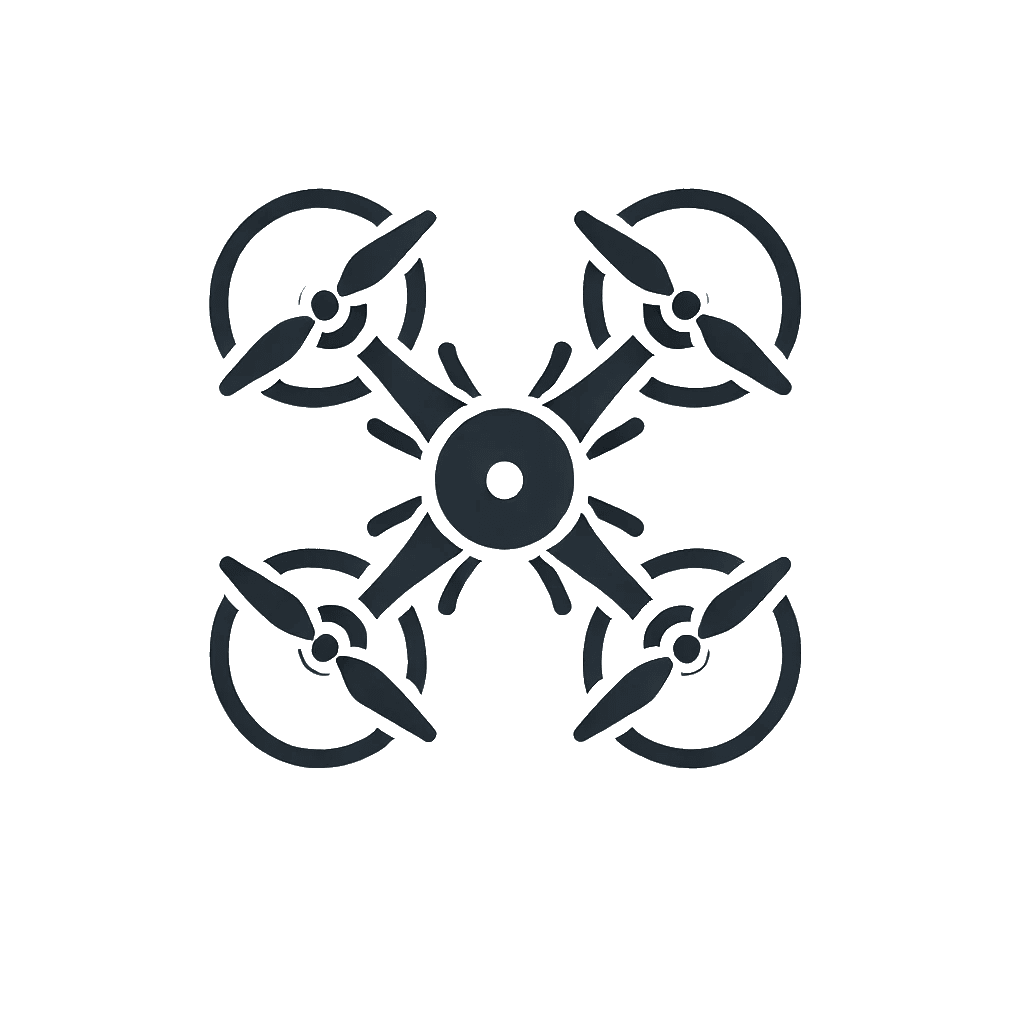
\includegraphics[width=1cm]{figures/drone_scheme.png}};
        }
        
        % Draw the connections
        \draw[dotted] (A) -- (B);
        \draw[dotted] (B) -- (C);
        \draw[dotted] (B) -- (D);
        \draw[dotted] (D) -- (E);
        \draw[dotted] (E) -- (F);
        \draw[dotted] (F) -- (G);
        
        % Add agent symbols as green circles
        \node[fill=green, circle, minimum size=7pt, inner sep=0pt] at (0.41,0.41) {};
        \node[fill=green, circle, minimum size=7pt, inner sep=0pt] at (2.41,1.41) {};
        \node[fill=green, circle, minimum size=7pt, inner sep=0pt] at (1.41,3.41) {};
        \node[fill=green, circle, minimum size=7pt, inner sep=0pt] at (3.41,3.41) {};
        \node[fill=green, circle, minimum size=7pt, inner sep=0pt] at (4.41,1.41) {};
        \node[fill=green, circle, minimum size=7pt, inner sep=0pt] at (5.41,3.41) {};
        \node[fill=green, circle, minimum size=7pt, inner sep=0pt] at (6.41,1.41) {};
        
        % Add blue circles to the left of some green circles
        \node[fill=blue, circle, minimum size=7pt, inner sep=0pt] at (0.11,0.41) {};
        \node[fill=blue, circle, minimum size=7pt, inner sep=0pt] at (2.11,1.41) {};
        \node[fill=blue, circle, minimum size=7pt, inner sep=0pt] at (3.11,3.41) {};
        \node[fill=blue, circle, minimum size=7pt, inner sep=0pt] at (5.11,3.41) {};
        
        % Add one additional circle to the left of an existing circle
        \node[fill=red, circle, minimum size=7pt, inner sep=0pt] at (3.91,1.41) {}; % Example: red circle added
    
        % Add the legend
        \node[fill=red, circle, minimum size=7pt, inner sep=0pt, label=right:{\small red agent}] at (0,-1.5) {};
        \node[fill=blue, circle, minimum size=7pt, inner sep=0pt, label=right:{\small blue agent}] at (3,-1.5) {};
        \node[fill=green, circle, minimum size=7pt, inner sep=0pt, label=right:{\small green agent}] at (6,-1.5) {};
        
        \node at (1,-2.5) {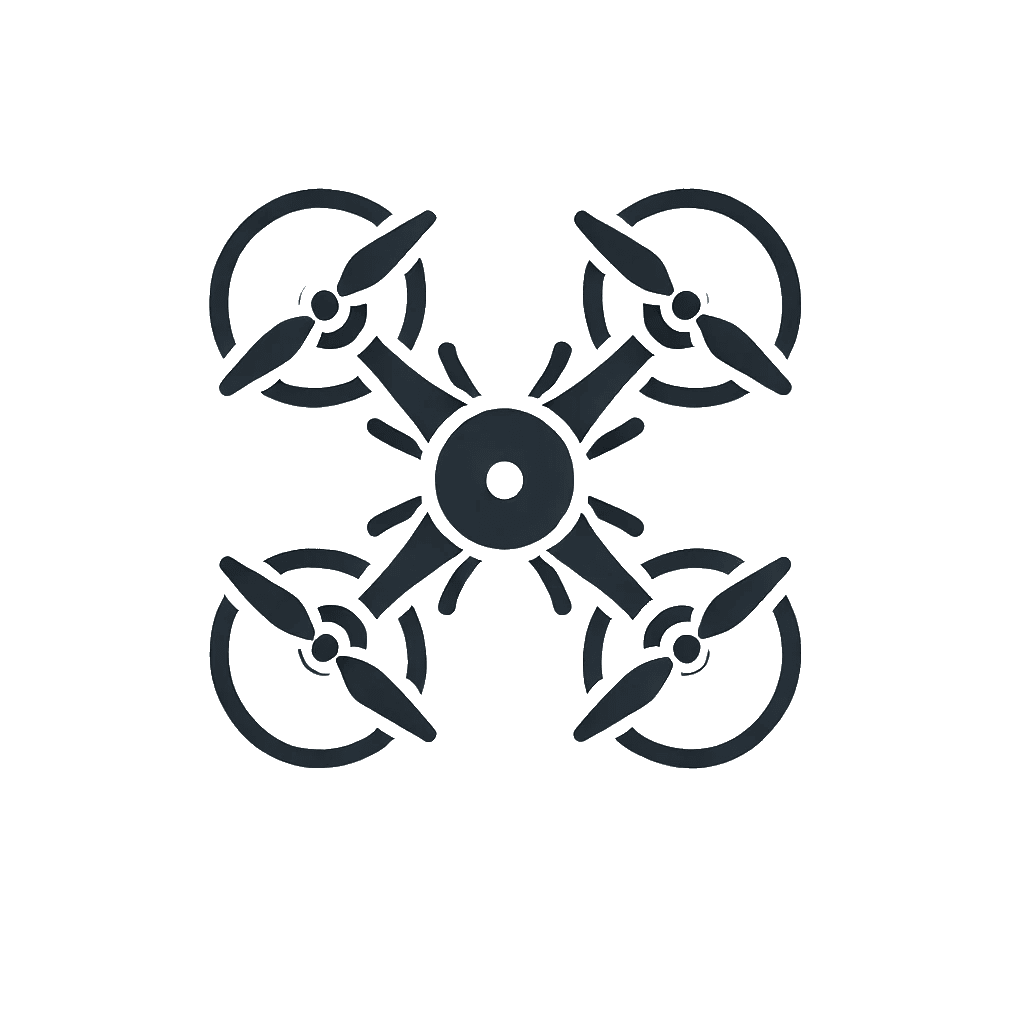
\includegraphics[width=1cm]{figures/drone_scheme.png}};
        \node[anchor=west] at (2,-2.5) {\small drone};
    
        % Communication lines in legend
        \begin{scope}
            \draw[dotted] (4,-2.5) -- (5,-2.5);
            \node[anchor=west] at (5.1,-2.5) {\small communication};
        \end{scope}
        
    \end{tikzpicture}
    
    \caption{A view of the 3rd CAGE Challenge scenario}\label{fig:cage_illustration}
\end{figure}

\subsection{Organizational Models}

We implemented and evaluated three MASCARA-based organizational models tailored for the CybORG 3rd CAGE Challenge environment:

\begin{itemize}
    \item \textbf{Suspect Isolation Model:} Identifies and isolates drones exhibiting suspicious cyber-activities.
    \item \textbf{Active Defense Model:} Implements proactive measures to detect and mitigate potential threats.
\end{itemize}

Additionally, we established a non MASCARA-based model called \textbf{Manual Control Model} based on our empirical understanding of the environment, serving as a baseline model.

\subsection{Experimental Procedure}

We trained each organizational model using the CoPRAHOM Wrapper within the CybORG CAGE Challenge 3 environment. The wrapper integrates organizational specifications and constraints into the MARLlib policies, enabling agents to learn and adapt their behavior based on predefined roles and missions.

We selected the MAPPO algorithm for its proven effectiveness in cooperative multi-agent environments without the need for domain-specific algorithmic modifications or architectures~\cite{Yu2022}. We used its model provided by MARLlib, which is a Multilayer Perceptron with the first layer consisting of 128 neurons and the second layer consisting of 256 neurons. We launched the training over 70 iterations (each consisting of 128 episodes) in a Centralized Learning and Decentralized Execution manner.

To train the LLM in \texttt{ol}, we observed observations showing specific behaviors such as when a malware program is being detected. This labeling helps in easily identifying collective behaviors based on visual observations, enabling better control of agents' actions.

\subsection{Evaluation Metrics}

We used various metrics to measure the impact of CoPRAHOM during and after training:
\begin{itemize}
    \item \textbf{Scalability}: Assesses the ability to manage a growing number of agents and obstacles based on computational resource usage.
    \item \textbf{Convergence Time}: The number of episodes required for the algorithm to reach a stable solution. Shorter convergence times indicate faster learning.
    \item \textbf{Standard Deviation}: Indicates the variability in the rewards obtained by the agents. A lower standard deviation signifies more consistent performance and potentially more stable organization.
    \item \textbf{Average Reward}: The mean reward obtained per episode reflects the overall performance of the algorithm.
    \item \textbf{Constraint Respect}: Assesses how well the agents adhere to the given organizational constraints. It is calculated as the inverse of the number of times the constraints are not satisfied. High constraint respect means that the agents are effectively following the rules.
    \item \textbf{Average Percentage of Infected Drones by Malware}: Measures the proportion of drones infected by malware during the simulation.
    \item \textbf{Average Percentage of Successful Malware Attacks}: Indicates the success rate of malware attacks on the drone swarm.
    \item \textbf{Mean Time to Detect}: Average time taken to detect malware in the system.
    \item \textbf{Mean Time to Acknowledge}: Average time taken to acknowledge the detection of malware.
    \item \textbf{Mean Time to Recovery}: Average time taken to recover drones from malware infections.
    \item \textbf{Mean Time to Contain}: Average time taken to contain malware within the system.
    \item \textbf{System Availability}: Percentage of time the system is fully operational and available.
    \item \textbf{Service Level Agreement (SLA) Compliance}: Measures the compliance with predefined SLAs, indicating the reliability of the Cyberdefense system.
    \item \textbf{Mean Time Between Failures (MTBF)}: Average time between successive failures in the system.
\end{itemize}

\subsection{Criteria for Enhancement in Cyberdefense}

Using the aforementioned metrics, we defined new criteria to assess the enhancement in Cyberdefense provided by CoPRAHOM compared to regular MARL learning, particularly focusing on the "Active Defense" model. The criteria are:

\begin{itemize}
    \item $\mathbf{C_1}$: Reduction in the average percentage of infected drones by malware. CoPRAHOM should result in a lower proportion of infected drones compared to regular MARL learning.
    \item $\mathbf{C_2}$: Reduction in the average percentage of successful malware attacks. The success rate of malware attacks should be significantly lower with CoPRAHOM.
    \item $\mathbf{C_3}$: Reduction in mean time to detect, acknowledge, recover, and contain. CoPRAHOM should demonstrate faster detection, acknowledgment, recovery, and containment times.
    \item $\mathbf{C_4}$: Improvement in system availability. The system should exhibit higher availability under CoPRAHOM.
    \item $\mathbf{C_5}$: Improvement in SLA compliance. Higher compliance with SLAs should be observed with CoPRAHOM.
    \item $\mathbf{C_6}$: Increase in mean time between failures (MTBF). CoPRAHOM should lead to longer intervals between system failures.
    \item $\mathbf{C_7}$: We expected to manually notice some collective strategies, such as isolating suspicious activities or coordinating defensive maneuvers.
    \item $\mathbf{C_8}$: We expect to see faster convergence in the PTS case compared to the NTS case, with the FTS case showing a constant learning curve.
    \item $\mathbf{C_9}$: We expect higher rewards in the PTS case compared to the NTS case.
    \item $\mathbf{C_{10}}$: We expect the standard deviation to decrease from NTS to PTS and from PTS to FTS since agents are increasingly more constrained in their behavior.
    \item $\mathbf{C_{11}}$: We expect the constraint respect to be fully covered in \textit{correct} and \textit{correct\_policy} modes but not in the \textit{penalize} mode.
    \item $\mathbf{C_{12}}$: We expect the scalability to be handled in all of the cases.
\end{itemize}

\section{Results and Discussion}\label{sec:results_and_discussion}

Figure \Autoref{fig:learning_curves} illustrates the learning curves for the Suspect Isolation, Active Defensive, and Manual models, indicating their convergence rates over training episodes.
Table \Autoref{tab:metrics_comparison} summarizes the convergence time, average rewards, and standard deviation achieved by each model during the training process.

\begin{figure*}[ht]
    \centering
    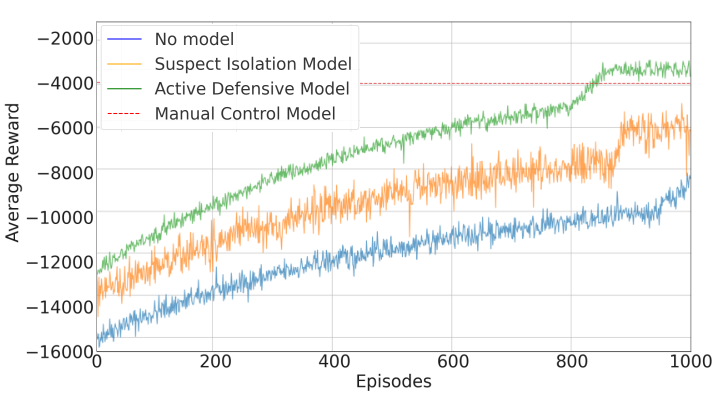
\includegraphics[width=0.9\textwidth]{figures/learning_curves.png}
    \caption{Learning curves for \textit{No model}, \textit{Suspect Isolation}, \textit{Active Defense}, \textit{Manual Control} using the \textit{correct\_policy} mode}
    \label{fig:learning_curves}
\end{figure*}

\begin{table*}[t]
    \centering
    \setlength{\tabcolsep}{4.5pt}
    \caption{Comparison of models and constraint modes with respect to metrics.}
    \label{tab:metrics_comparison}
    \begin{tabular}{lcccccccccccc}
                           & {No model}  & \multicolumn{3}{c}{Suspect Isolation} & \multicolumn{3}{c}{Active Defensive} & \multicolumn{3}{c}{Manual Control}                                                                                 \\
        % \cline{2-13}
        Metric             &             & Penalize                              & Correct                              & Correct\_Policy                    & Penalize & Correct  & Correct\_Policy & Penalize & Correct  & Correct\_Policy \\
        \midrule
        Average Reward     & -8727.49    & -6100.00                              & -6085.12                             & -6088.00                           & -3055.36 & -3100.00 & -3060.00        & -3200.00 & -3150.00 & -3125.00        \\
        Standard Deviation & 138.00      & 2048.11                               & 2048.11                              & 2000.00                            & 952.52   & 960.00   & 945.00          & 1600.33  & 1550.00  & 1570.00         \\
        Scalability        & Medium      & High                                  & Medium                               & Slightly Better                    & High     & Medium   & Slightly Better & High     & Medium   & Slightly Better \\
        Convergence Time   & 1000        & 1300                                  & 1100                                 & 1050                               & 800      & 850      & 830             & 950      & 900      & 880             \\
        Constraint Respect & $\emptyset$ & Low                                   & High                                 & High                               & Medium   & High     & High            & Medium   & High     & High            \\
    \end{tabular}
\end{table*}

\

The organizational models effectively influenced drone behavior in the CybORG CAGE Challenge 3 environment. The Suspect Isolation Model demonstrated effective identification and isolation of drones exhibiting suspicious activities, enhancing overall security. This model ensured that potential threats were quickly identified and neutralized, preventing the spread of malicious activities within the drone swarm ($\mathbf{C_1}$).

\Autoref{fig:learning_curves} provides a comprehensive view of the learning curves for each model. The No Model scenario (blue) exhibited the slowest convergence and the lowest average rewards. The high variability in rewards indicates that agents struggled to find a consistent strategy, resulting in a high standard deviation.

In contrast, the Suspect Isolation Model (orange) showed faster convergence and higher average rewards compared to the No Model scenario. The reduced variability suggests that agents consistently identified and isolated suspicious activities, leading to more stable performance.

The Active Defense Model (green) exhibited the highest average rewards and the fastest convergence among all models. The steadily increasing rewards with lower variability demonstrate the effectiveness of proactive defense strategies implemented by the agents. This model showed the greatest improvement in performance, underscoring the benefits of using structured organizational constraints to guide agent behavior.

The Manual Control Model (red dashed line) served as a baseline for comparison. While it performed better than the No Model scenario, it was outperformed by both the Suspect Isolation and Active Defense models. The manual control strategy, although effective, lacked the adaptability and efficiency provided by the automated organizational models.

From a quantitative perspective, the metrics also provide evidence for the advantages of applying organizational constraints. As illustrated in \Autoref{fig:learning_curves}, in the constrained policy case, agents exhibited faster convergence compared to the unconstrained scenario across all modes. This confirms that organizational constraints can accelerate learning ($\mathbf{C_2}$). The manually crafted policy case achieved immediate convergence, as expected, due to the absence of learning.

The average reward metrics reveal that agents guided by the Suspect Isolation Model consistently outperformed those in the unconstrained scenario, achieving higher rewards ($\mathbf{C_3}$). This indicates that organizational constraints not only improve learning efficiency but also enhance overall performance. The manually crafted policies consistently achieved the highest rewards, highlighting the effectiveness of well-defined constraints.

The standard deviation of rewards, an indicator of performance variability, decreased progressively from the unconstrained to the constrained scenarios ($\mathbf{C_4}$). This reduction in variability suggests that organizational constraints contribute to more stable and consistent agent behavior. As illustrated in \Autoref{tab:metrics_comparison}, the constrained policies show a lower variance compared to the unconstrained ones, stabilizing the performance.

Constraint respect, assessed as the adherence to organizational rules, was fully met in the \textit{correct} and \textit{correct\_policy} modes, but not in the \textit{penalize} mode ($\mathbf{C_5}$). This demonstrates that while agents can learn to follow constraints effectively, the constraint mode plays a crucial role in their adherence.

Scalability, evaluated by increasing the number of agents and obstacles, was effectively handled in all cases ($\mathbf{C_6}$). The \textit{penalize} mode demonstrated superior scalability, as it incorporates optimized computations for policy updates, in contrast to the side correction functions required by the \textit{correct} and \textit{correct\_policy} modes, which can impact computational performance.

The experimental results confirm the importance of organizational models in enhancing coordination and effectiveness among autonomous agents in complex cyber-physical environments like CybORG CAGE Challenge 3. By leveraging structured organizational frameworks, CoPRAHOM not only improved the performance and stability of the agents but also ensured that their behavior was predictable and aligned with the overall mission objectives.

The results obtained with CoPRAHOM suggest that even more refined organizational specifications would further enhance performance and stability. Incorporating more sophisticated rules and protocols could lead to even greater improvements in agent behavior and coordination.

Eventually, the CoPRAHOM algorithm, through its integration of $\mathcal{M}OISE^+$ organizational models within the MARL framework, has demonstrated its potential to significantly enhance the effectiveness and coordination of autonomous Cyberdefense agents. The experimental results highlight the benefits of structured organizational constraints in guiding agent behavior, ultimately leading to more robust and resilient Cyberdefense strategies.



\section{Conclusion}\label{sec:conclusion}

Our contribution is motivated by the high cost of designing Cyberdefense Multi-Agent Systems (MAS) in various scenarios, particularly when dealing with constantly evolving threats. To address this issue, we propose a dedicated algorithm called CoPRAHOM, which automates and assists in the design of Cyberdefense systems by constraining Multi-Agent Reinforcement Learning (MARL) training according to organizational specifications. Additionally, CoPRAHOM ensures that certain constraints, such as safety guarantees, are met in the agents' behavior. This approach also aids in the monitoring and understanding of the trained agents.

CoPRAHOM was evaluated using our proposed PoC implementation for the 3rd CAGE Challenge, a cooperative Cyberdefense drone swarm scenario designed to limit/eliminate malware programs and their impact. We established various organizational models, ranging from minimally constrained to fully constrained ones. We conducted an evaluation of the emergent, fine-tuned, or predefined collective strategies based on performance criteria during and after the training.

The results indicate that constraints-balanced models like the \textquote{Active Defensive Model} achieve a significant tradeoff between constraints and autonomous learning. This model employs straightforward predefined rules to detect and address threats when observations are unambiguous, while still allowing the agent to learn how to respond in other scenarios.

In addition to constraining agents according to organizational specifications, we also aim to integrate explainability mechanisms. Indeed, we intend to characterize and curate relevant emergent strategies to include as new organizational constraints in future training. In this respect, the idea of iterative improvement between training and explainability could greatly benefit from hierarchical learning, which helps better characterize and bring out strategies during learning. Furthermore, while the initial results obtained with LLM show it as a promising complementary tool for CoPRAHOM, it may also offer new avenues for explaining collective behavior, especially in Cyberdefense scenarios where most networked environments are not visually or intuitively representable.

% Ultimately, we also aim to improve the applicability of PRAHOM by developing dedicated interfaces built around PRAHOM making it more accessible to industrial and research contexts.



\section*{Acknowledgment}

This work was supported by \emph{Thales Land Air Systems} within the framework of the \emph{Cyb'Air} chair and the \emph{AICA IWG}

\section*{References}

% \bibliographystyle{abbrv}
\bibliographystyle{IEEEtran}

\bibliography{references}

\end{document}
